\chapter{国内外相关研究现状}\label{chap:related_work}

目前,国内外针对从非结构化文本中进行需求发现和提取已经有一些研究成果。
% 在许多开源和工业项目中,开发人员大量使用书面沟通渠道,例如邮件列表,issue tracker、聊天工具等,并且这样的方式已经遍布全球开发人员的日产工作中。
通过应用一些自然语言处理技术和文本挖掘如情感分析、话题建模、机器学习等技术,研究人员可以对这些非结构化文本进行意图分类,分类为如缺陷报告、解决方案、需求等类别\cite{maalej2015bug},其中识别到的需求可以服务于发布计划工具、向应用开发者提供支持,并决定哪些新功能需要在下个版本中实现。本章主要从隐藏需求对话识别工具构建过程中所涉及的相关概念以及技术细节,包括基于文本数据的需求发现、聊天对话文本在软件工程中的应用、文本分类以及少样本学习几方面进行探究并介绍国内外相关研究工作。

\section{基于文本数据的需求发现}


目前,人工和自动分析比如基于规则的方法以及有监督的机器学习方法正在被大量应用在分析对软件工程师和非专家的利益相关者有用的信息,如需求等信息中\cite{Morales2019Speech},并已有大量相关的研究工作。
\subsection{基于手工规则的需求发现}

RE Vlas等人\cite{morales2014discovering}提出一种基于语法的需求发现工具。作者使用Subject-Action-Object(SAO)语法标签对需求进行解析和表示。其中subject是需求声明的发出者,action定义了需求里面定义的特征,object表示被action影响的对象。比如:“这个提交按钮应该把表单数据提交给处理组件”中,“提交按钮”是subject,“发送”是action,object是“表单数据”。图\ref{fig:sao}是SAO方法对密码安全特征需求进行识别的一个例子。
\begin{figure}[htbp]
    \centering
    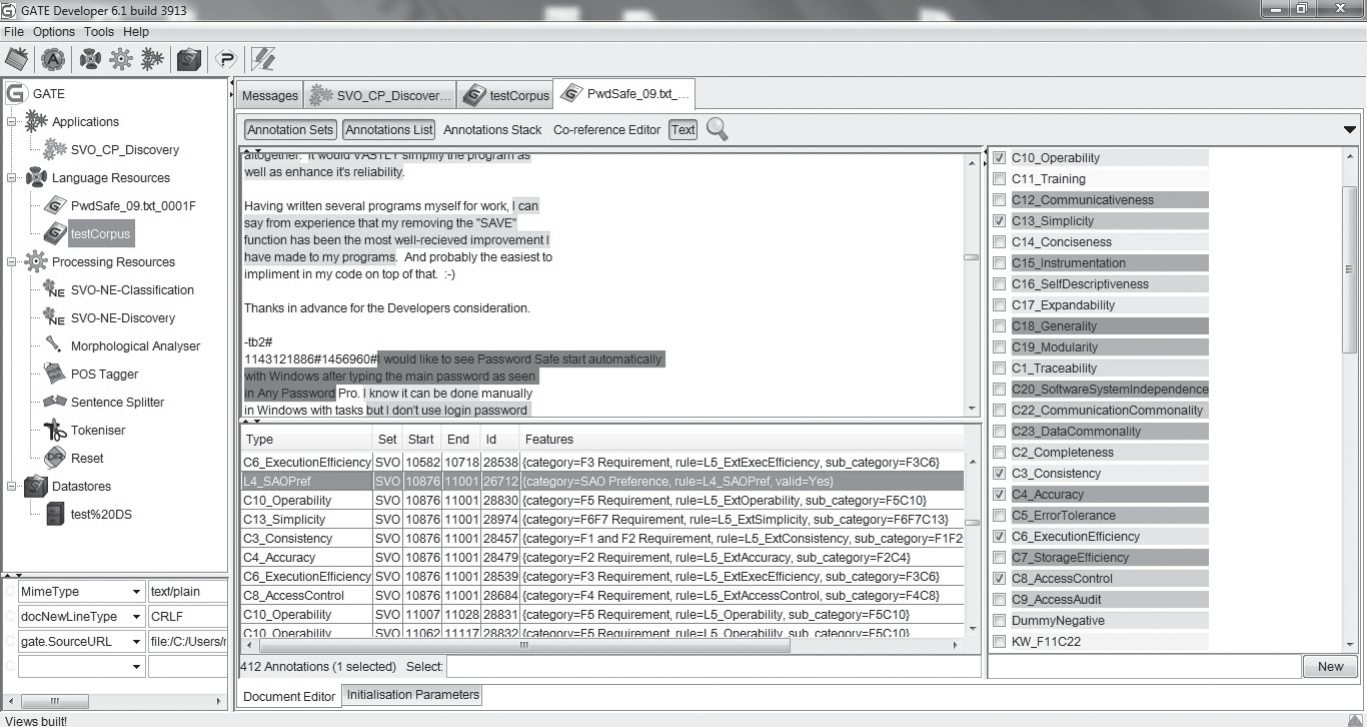
\includegraphics[width=0.70\textwidth]{Img/sao.png}
    \bicaption{基于SAO方法对密码安全特征需求进行识别}{SAO-based Recognized Password Safe Feature Requirements}
    \label{fig:sao}
\end{figure}


邮件是开发者之间进行沟通的重要方式之一,通常包含需求、观点询问、问题发现、解决方案、信息提供等不同类别的信息。Di Sorbo等人\cite{Sorbo2016Development}提出一种名叫DECA(开发者电子邮件内容分析器)的半监督学习方法,通过使用自然语言解析工具分析文本的语言学特征并且从询问帮助、提供帮助、提出新需求、报告或者讨论BUG等几方面对开发者的意图进行分类。Di Sorbo等人首先根据来自Ubuntu和QT的数据设置更适合邮件列表信息的分类,具体分类类别如表\ref{tab:deca0}所示。
\begin{table}[htb]
\bicaption{句子例子以及对应的类别}{Sentence examples and corresponding categories}
    \label{tab:deca0}
    \centering
    \footnotesize% fontsize
    \setlength{\tabcolsep}{4pt}% column separation
    \renewcommand{\arraystretch}{1.2}%row space 
\begin{tabular}{lcccccccc}
\hline
句子类别的例子      & 分类类别 \\
\hline
讨论一个变更       & 需求 \\
定位BUG        & 问题发现 \\
BUG是否被修复     & 信息询问 \\
针对已知问题提出解决方案 & 解决方案 \\
请求其他开发者做出变更  & 需求 \\
询问代码时如何工作的   & 信息询问 \\
询问为何这样写代码    & 信息询问 \\
向某人征求意见      & 意见询问 \\
找出代码作者       & 信息询问 \\
更多的了解代码      & 信息询问 \\
告诉其他开发者一些事情  & 信息提供 \\
\hline
\end{tabular}
\end{table}
然后对其进行手工标注,作者发现开发人员在关于开发问题的讨论中撰写关于现有错误或者建议提出需求时,他们倾向于使用一些经常性的语言模式,比如对于“我们可以使用漏桶算法来限制带宽”,可以发现句子中提供一个明确定义的谓词-参数结构,对此,可以看出大多数具有谓词-论元结构的句子表明解决方案。作者定义了启发式规则,首先发现句子的特定句法结构,然后推广某些类型的信息,最后忽略无用的信息。所以,作者定义了“【某人】可以使用【某事物】”的一般模式来识别解决方案。图\ref{fig:deca1}是作者通过斯坦福依存句法分析来分析启发式规则时的例子。
\begin{figure}[htb]
    \centering
    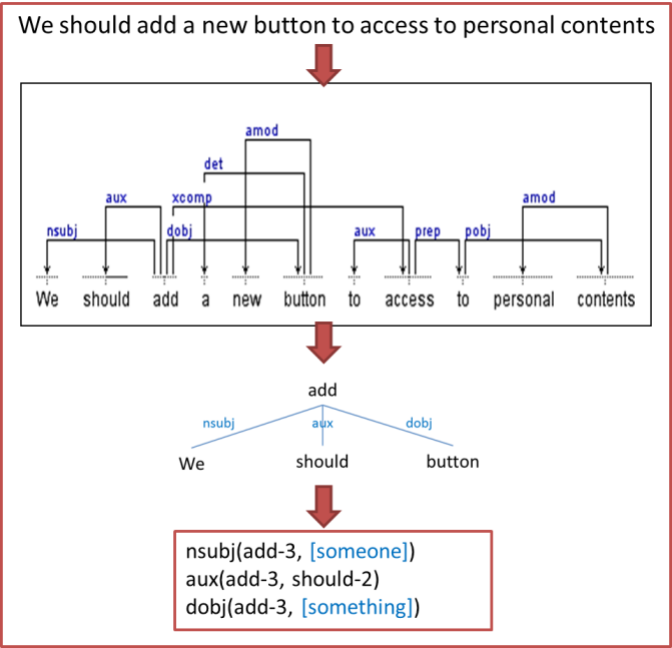
\includegraphics[width=0.60\textwidth]{deca1}
    \bicaption{需求文本中的自然语言解析树}{Natural language parsing tree about feature request}
    \label{fig:deca1}
\end{figure}
作者通过图\ref{fig:deca1}定义了“【某人】应添加【某事物】”的启发规则并于需求相关联。Andrea Di Sorbo等人的观点是在软件工程领域存在相关的重复语言模式,这对软件过程中的需求分析非常有用。

L Shi等人\cite{shi2017understanding}提出利用自然语言处理技术生成一组模糊规则来自动分析需求的方法,其将需求中的每个句子进行分类,类别有意图、解释、益处、缺点、示例和无关,分类的结果用来增量生成模糊规则。作者定义了这些类别以及类别的定义和优先级来帮助结构化表示需求,并重点显示值得关注的内容,如表\ref{tab:fra0}所示。
\begin{table}[htb]
\bicaption{句子类别的定义}{Definitions of sentence categories}
    \label{tab:fra0}
    \centering
    \footnotesize% fontsize
    \setlength{\tabcolsep}{4pt}% column separation
    \renewcommand{\arraystretch}{1.2}%row space 
\begin{tabular}{lcccccccc}
\hline
类别 & 重要性 & 定义                     \\
\hline
意图 & 1   & 关于改进系统和功能的主意、需求、期望的描述  \\
益处 & 2   & 关于提出的需求带来的好处和有帮助的结果的描述 \\
缺点 & 3   & 关于当前系统行为的缺点            \\
例子 & 4   & 关于支持提出的需求的例子           \\
解释 & 5   & 关于提出需求的场景和解决           \\
无关 & 6   & 和系统无关的信息              \\
\hline
\end{tabular}
\end{table}
作者分别在词汇、语法、语义三个级别启发式地定义模糊规则。词汇通过设置不同类别句子的词汇表来对句子进行分类,句法通过对句子进行依存结构分析不同句子类别的句法特征,语义层面通过定义在某个类别的句子中的语言表达的含义,如图\ref{fig:fra1}所示的语义模式。
\begin{figure}[htb]
    \centering
    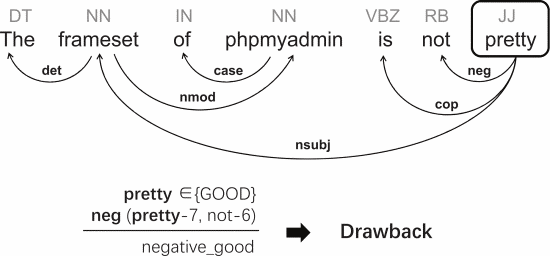
\includegraphics[width=0.70\textwidth]{fra1}
    \bicaption{缺陷类别的语义模式示例}{An example about semantic pattern of defect class}
    \label{fig:fra1}
\end{figure}
实验表明,随着新规则的引入,模糊规则的分类性能越来越高。此外,在将模糊规则转换成布尔变量之后,将其应用于各种机器学习算法上得到了更好的效果。

I Morales-Ramirez等人\cite{Morales2019Speech}关注于分析在线讨论,如开源软件的邮件列表和用户论坛,在这里,不同的利益相关者比如开发者、软件终端用户会讨论有助于软件发展的信息。基于规则Speech-acts分析\cite{morales2014discovering}用在线讨论的自动分析上,比如可以通过学生的查询理解学生的意图\cite{feng2006intelligent}等。 Speech-acts理论认为当某人说一些话存在一些模式让对方相信或者做出对应的行为\cite{acts1969essay},比如在询问一个新功能中使用的词汇模式包括:“添加特征”、“想要这个特征”等。作者把不同speech-acts规则归为几类:c-Assertive, c-Responsive, c-Requestive和c-Attachment。如表\ref{tab:speech-act0}所示,每一列为对应的独立speech-acts类别。
\begin{table}[htb]
\bicaption{Speech-acts列表}{List of speech-acts}
    \label{tab:speech-act0}
    \centering
    \footnotesize% fontsize
    \setlength{\tabcolsep}{4pt}% column separation
    \renewcommand{\arraystretch}{1.2}%row space 
\begin{tabular}{lcccccccc}
\hline
c-Assertive & c-Requestive & c-Responsive & c-Attachment & c-Other          \\
\hline
断定        & 请求         & 回应         & 附件         & 描述性的      \\
确认        & 需求         & 建议         & 代码         & 接受           \\
让步        & 问题         & 支持         & URL链接      & 拒绝           \\
            &              &              & 日志文件     & 消极观点 \\
            &              &              &              & 积极观点  \\
            &              &              &              & 感谢            \\
            &              &              &              & 内容丰富的 \\
\hline            
\end{tabular}
\end{table}
基于Speech-acts的模型结构如图\ref{fig:speech-acts1}所示。
\begin{figure}[htb]
    \centering
    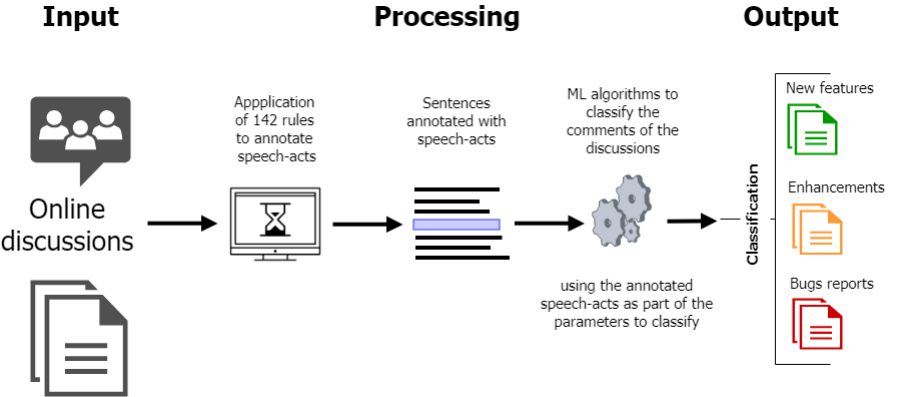
\includegraphics[width=0.70\textwidth]{Img/speech-acts1.png}
    \bicaption{基于Speech-acts的分析模型}{Speech-acts based analysis approach}
    \label{fig:speech-acts1}
\end{figure}
这个工具结合了作者关于需求的知识,以及利益相关者在在线讨论中表达需求的方式来定义142条词法-句法规则,从而对需求进行识别。

\subsection{基于统计机器学习的需求发现}
开发者和客户通常会通过会议来获取用户故事,P Rodeghero等人\cite{Rodeghero2017Detecting}提出一种从客户和开发人员之间记录的对话中自动提取和用户故事相关信息的方法。作者从对话记录中自动提取用于构建用户故事的数据,分别进行定性研究,其可以检验对话中包含用户故事的角色、功能和基本原理的假设;以及定量研究以确定现有分类算法的效果。通过定性研究分析得到大约5.5\%的对话包含功能信息,2.9\%包含了基本原理,只有0.5\%讨论了角色,发现对话包含重要的功能和基本原理信息,但关于角色的数据非常有限。作者训练了一个分类器用于检测包含功能数据的对话部分。在数据收集部分,作者收集一家软件开发公司的会议记录,并标注文件名、会话、摘要、会话转折、角色、功能、理由等信息,对会议记录提取了25个属性进行分类,分析的单位是转折而不是句子,提出的方法模型如图\ref{fig:Rodeghero2017Detecting}所示。
\begin{figure}[htb]
    \centering
    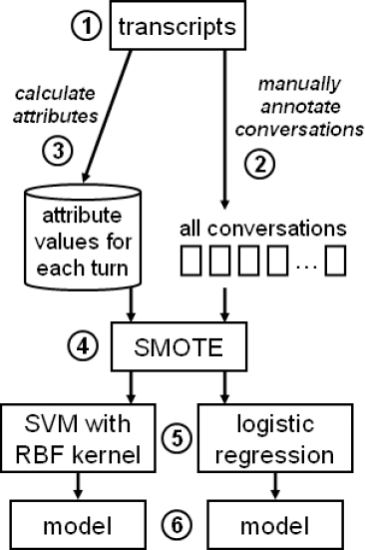
\includegraphics[width=0.40\textwidth]{Rodeghero2017Detecting.png}
    \bicaption{分类器模型结构图}{Structure of classifier}
    \label{fig:Rodeghero2017Detecting}
\end{figure}

Q Huang等人\cite{Huang2018Automating}发现Di Sorbo等人的分类类别还有55\%的句子不能覆盖,于是在其分类的基础上合并了两种意图,并新增了两种意图,提炼过的分类类别如表\ref{tab:aim0}所示。
\begin{table}[htb]
\bicaption{精炼后的意图分类}{Intention classification after refine}
    \label{tab:aim0}
    \centering
    \footnotesize% fontsize
    \setlength{\tabcolsep}{4pt}% column separation
    \renewcommand{\arraystretch}{1.2}%row space 
\begin{tabular}{lcccccccc}
\hline
类别   & 描述                 \\
\hline
信息提供 & 将知识、经验、计划、更新共享给其他人 \\
信息寻找 & 希望得到信息和帮助          \\
需求 & 帮助改进现有功能或提出新功能     \\
解决方案 & 共享可能的解决方案          \\
问题发现 & 报告BUG,或描述异常行为      \\
侧面评价 & 表达观点或进行评价          \\
无意义  & 无意义的或不重要的         \\
\hline
\end{tabular}
\end{table}
并提出了使用Convolutional Neural Network(CNN)\cite{kim2014convolutional}的方法自动将句子分类为不同的意图类别,整体模型架构如图\ref{fig:aim1}所示。
\begin{figure}[htbp]
    \centering
    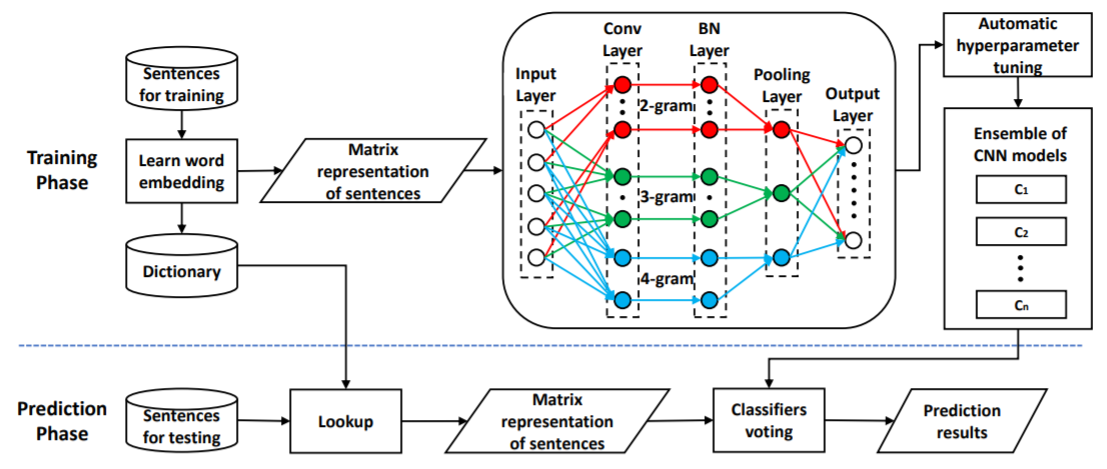
\includegraphics[width=0.8\textwidth]{aim1.png}
    \bicaption{CNN分类模型整体框架}{Structure of CNN classifier}
    \label{fig:aim1}
\end{figure}
CNN将句子作为输入,输出7个概率值,从而得出概率最大的句子类别,即使测试集中没有出现和训练集相似的模式或者关键词,模型也会给出概率最大的类别,从而覆盖所有句子。

% Y Zhang等人\cite{zhang2015sensitivity}发现词向量的维度、过滤器的数量以及过滤器的深度是对效果影响较大的超参数,作者使用贪婪的方式搜索最优参数。
D Arya等人\cite{arya2019analysis}通过对15个问题讨论进行内容定量分析,确定了包括潜在需求在内的16种信息类型。作者手工构建了14个对话特征,并使用随机森林作为分类器,对表达新需求的句子可以达到66\%的F1值。
W Maalej等人\cite{maalej2015bug}使用自然语言处理技术包括文本分类、情感分析把App Reviews分类为缺陷报告、需求、用户经验和打分。其中分类结果的precision可达到70-95\%,recall可达到80-90\%。

\section{聊天对话文本在软件工程中的应用}
在各种软件开发项目中,两种常见的聊天方式为同步和异步沟通方式\cite{yu2011communications}。同步方式包括Internet Relay Chat(IRC)等聊天工具,异步方式包括邮件列表、issue tracker等工具。
% 目前已有大量的研究工作正在开发有效的工具支持软件分析,它们利用自然语言处理技术从应用商店评论、在线聊天记录、邮件列表、用户论坛等文本数据中抽取相关信息,并且使用文本挖掘和机器学习技术对信息进行分类如缺陷报告或者需求。
其中基于Web平台的关于软件应用和服务的在线聊天讨论中包含着关于软件系统的丰富的信息,并在包括需求发现等各种软件工程任务中表现出来巨大的价值\cite{Morales2019Speech}。

B Lin等人\cite{lin2016developers}通过一项关于开发者怎么使用Slack、哪个聊天工具在开源社区比较流行、聊天工具能够为软件开发带来怎么样的好处的研究,发现开发者使用Slack进行个人、团队、社区级别的交流,Slack也占据越来越重要的地位,在某些情况下会代替邮件。
E Shihab等人\cite{shihab2009studying}通过两个大型开源项目从几个维度分析了开发者IRC会议:会议内容、会议参与者、他们的贡献、会议类型。作者的研究表明IRC正在开源社区占据越来越重要的地位,强调了从开发者聊天记录中可以获取丰富的信息。
P Chatterjee等人\cite{chatterjee2019exploratory}调查了通过挖掘开发者谈话从而支持软件维护和演化的有效性和挑战性,作者发现开发者倾向于通过即时聊天工具分享对于观点或者有意义的想法,并且说明了通过应用一些技术和训练集可以达到较高的对话解耦效果。



\section{文本分类方法}
\subsection{朴素贝叶斯}
朴素贝叶斯(Naive Bayesian)\cite{mccallum1998comparison}是基于词袋假设和贝叶斯公式的常用文本分类模型。对于文档$d$和类别$c$,该文档属于类别$c$的概率为$P(c|d)=\frac{P(d|c)P(c)}{P(d)}$,其极大后验也即最有可能的类别为$c_{MAP}=\mathop{\arg\max}\limits_{c \in C}P(c|d)$,去掉贝叶斯公式分母可得$c_{MAP}=\mathop{\arg\max}\limits_{c \in C}P(d|c)P(c)$,基于词袋模型和特征条件独立性假设可得
$$c_{NB}=\mathop{\arg\max}\limits_{c \in C}P(x_1|c)P(x_2|c)\dots P(x_n|c)P(c)=\mathop{\arg\max}\limits_{c \in C}p(c)\prod\limits_{x \in X}P(x|c)$$
因此,通过极大似然估计获得似然概率$P(x|c)$和先验概率$P(c)$即可得到后验概率$P(c|d)$,然后将后验最大的类别作为分类结果。

\subsection{fastText}
fastText\cite{joulin2016bag}是Facebook开源的一个词向量计算和文本分类工具。
% ,其优点主要在于在文本分类任务中,fastText(浅层网络)往往能取得和深度网络相媲美的精度,却在训练时间上比深度网络快许多数量级。在标准的多核CPU上,能够在10分钟之内训练10亿词级别语料库的词向量,在1分钟之内能够分类有30多万类别的50多万条句子。
其模型架构和word2vec\cite{mikolov2013distributed}的CBOW模型架构非常相似,图\ref{fig:fasttext}所示为fastText的模型结构图。
\begin{figure}[htb]
    \centering
    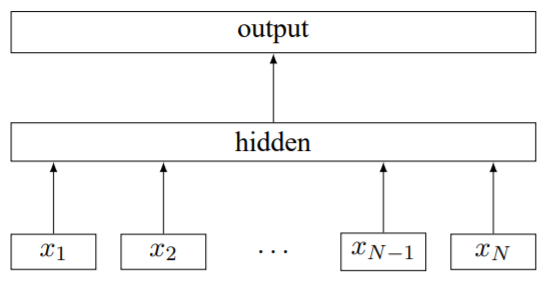
\includegraphics[width=0.6\textwidth]{Img/fastText.png}
    \bicaption{对于具有N ngram句子特征$x_1, \dots , x_N$ 的句子的fastText模型结构。特征被嵌入表示并且求平均来作为隐藏特征}{Model architecture of fastText for a sentence with N ngram features $x_1, \dots , x_N$ . The features are embedded and averaged to form the hidden variable}
    \label{fig:fasttext}
\end{figure}
fastText模型结构类似于CBOW只有三层,并且也利用了分层的Softmax减少训练时间。但是CBOW的输入是目标单词的上下文窗口,fastText的输入是用来表示单个文档的多个单词及其n-gram特征。CBOW的输出是目标词汇,fastText的输出是文档对应的类别。并且fastText将单词的字符级别的n-gram向量作为输入的额外特征。

\subsection{随机森林}
随机森林(Random Forest)\cite{liaw2002classification}
随机森林是一种集成机器学习中Bagging的方法,其是由很多决策树构成的,不同决策树之间是独立的。如图\ref{fig:rf-model}所示,当进行分类任务时,对于新的输入样本,森林中的每一棵决策树对其分别进行判断和分类,每个决策树会得到一个自己的分类结果,决策树的分类结果中哪一个分类最多,那么随机森林就会把这个结果当做最终的结果。
\begin{figure}[htb]
    \centering
    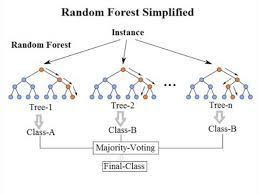
\includegraphics[width=0.6\textwidth]{Img/rf-model.jpg}
    \bicaption{随机森林模型架构}{Model architecture of Random Forest}
    \label{fig:rf-model}
\end{figure}
它的构造过程首先对数据集合进行有放回的抽取,得到若干个子数据集,对于每个数据集中随机选取的特征,使用信息增益进行分裂,然后得到若干树组成森林。由于随机森林选取数据集和特征的随机性,其优点在于不容易过拟合,处理很高维度的数据,并且不用做特征选择,由于决策树并行生成,因此可以并行训练。

\subsection{梯度提升决策树}
梯度提升决策树(Gradient Boosting Decision Tree)\cite{ke2017lightgbm}
梯度提升树是另一种基于树的集成机器学习方法,其模型定义为加法模型:
$$f_M(x)=\sum^M_{m=1}\alpha_mh_m(x,\theta_m)=\sum^M_{m=1}f(x,\theta_m)$$,其中$h_m$是第m棵树,$\alpha_m$是第m棵树的权重。GBDT目标函数为:
$$\large {r_{mi}} = -\left[\frac{\partial L(y_i,f(x_i))}{\partial f(x_i)} \right]_{f(x)=f_{m-1}(x)}$$,使用平法误差损失函数时$L(y, f(x)) = (y-f(x))^2$。其使用经验风险最小化求得下棵树的参数:
$$\hat \theta_{m} = \mathop{\arg\min}\limits_{\theta_{m}} \sum_{i=1}^ML(y_{i}, f_{m-1}(x_{i})+T(x_{i}; \theta_{m}))$$

\section{少样本学习}
深度学习在计算机视觉和NLP领域都取得了巨大的成功。但是它严重依赖于足够多的训练数据量,并且当标记的资源不足时,很难达到很好的效果。

基于在线聊天消息的自动挖掘技术面临标注资源不足的问题,在在线聊天中,开发人员会在短时间内创建大量的讨论对话。为了学习有效的模型,需要从这些大量讨论文本中标注对话数据,这是一项非常耗时的工作,因为这些对话数据不仅文本很长、掺杂大量无关信息,而且标注人员还需要有领域知识来对对话进行充分的理解。

对此类标注数据困难的情况,少样本学习被提出来克服这些问题\cite{wang2019few},其旨在通过学习少量样本以及对应的标签信息从而对提高对新样本的学习能力。少样本学习可以分为以下三类\cite{chen2019closer}:基于模型的方法:其旨在通过模型设计出发,从少量标注数据的分类任务中学习映射函数;基于优化的方法:其可调整传统的梯度下降优化器方法以拟合数据分布;基于度量的方法:其通过学习相似性度量函数对样本进行分类。

\subsection{基于模型的少样本学习方法}
A Santoro等人\cite{santoro2016one}提出的使用记忆增强的方法来解决少样本问题是基于模型方法的一个代表。由于神经网络图灵机(NTMs)能通过外部存储(external memory)进行短时记忆,并能通过缓慢参数更新来进行长时记忆,文章使用NTM来存储样本以及对应类别表示信息,当需要预测一个已经模型已经见过的样本时,这些信息可以相应的被检索,因此,文章方法可以快速准确地预测那些只出现过一次的数据。另一方面,如图\ref{fig:few-memory}所示,文章模型基于RNN结构,
\begin{figure}[htb]
    \centering
    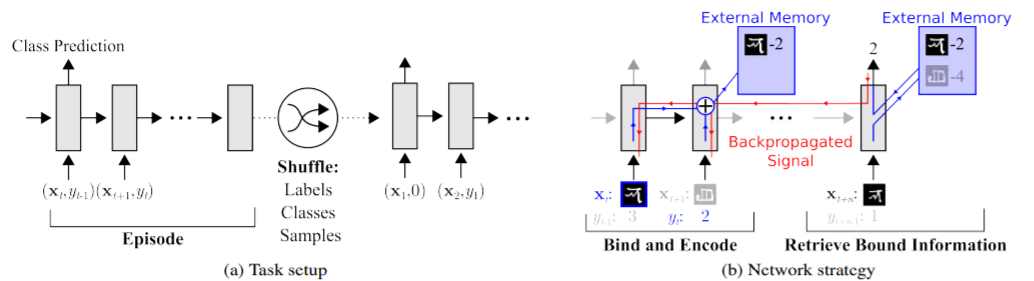
\includegraphics[width=0.8\textwidth]{Img/few-memory.png}
    \bicaption{基于外部知识模块的少样本学习方法}{The approach of few-shot learning based on external memory module}
    \label{fig:few-memory}
\end{figure}
模型将数据看成序列来进行训练,训练过程中将样本和标签对应,并更新外部知识模块,在测试时输入新的类的样本进行分类时,模型可以把未出现过的数据连接到对应相关的外部记忆模块中的表示,借助外部知识信息达到更好的分类效果。

\subsection{基于优化的少样本学习方法}
C Finn等人\cite{finn2017model}提出了一种模型无关的元学习方法,其可以快速拟合多种不同的包括分类、回归和强化学习等任务。文章的方法可以在小量样本上,用少量的梯度更新步骤来训练模型的初始化参数,从而可以获得较好的泛化性能,并且容易对模型进行微调。具体的,如图\ref{fig:few-optim}所示,该方法能够找对任务的损失函数敏感的参数$\theta$,
\begin{figure}[htb]
    \centering
    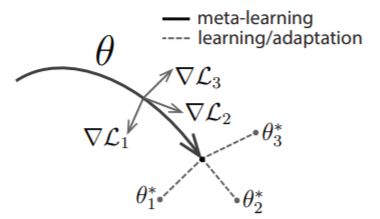
\includegraphics[width=0.6\textwidth]{Img/few-optim.png}
    \bicaption{模型无关的元学习算法}{The algorithm of Model-Agnostic Meta-Learning}
    \label{fig:few-optim}
\end{figure}
对参数$\theta$进行微小改变便能较大程度改善模型的损失函数、适应于不同任务并提高任务效果。



\subsection{基于度量的少样本学习方法}
孪生网络\cite{bromley1994signature}是一种基于度量的少样本学习技术,该技术被广泛用于衡量文本或图像之间的语义相似性\cite{mueller2016siamese}。传统的分类模型尝试学习从单个实例映射到其类别的函数空间,但是当可用的标注资源数据较少时,这些分类模型不能达到理想的效果。与传统方法不同,孪生网络将成对的实例作为输入,旨在学习来决定两个实例是否属于同一类别的关键特征。如图\ref{fig:siamese-model}所示,它由两个相同的子模块组成,这些子模块不仅共享模型结构,而且还共享参数。
\begin{figure}[htb]
    \centering
    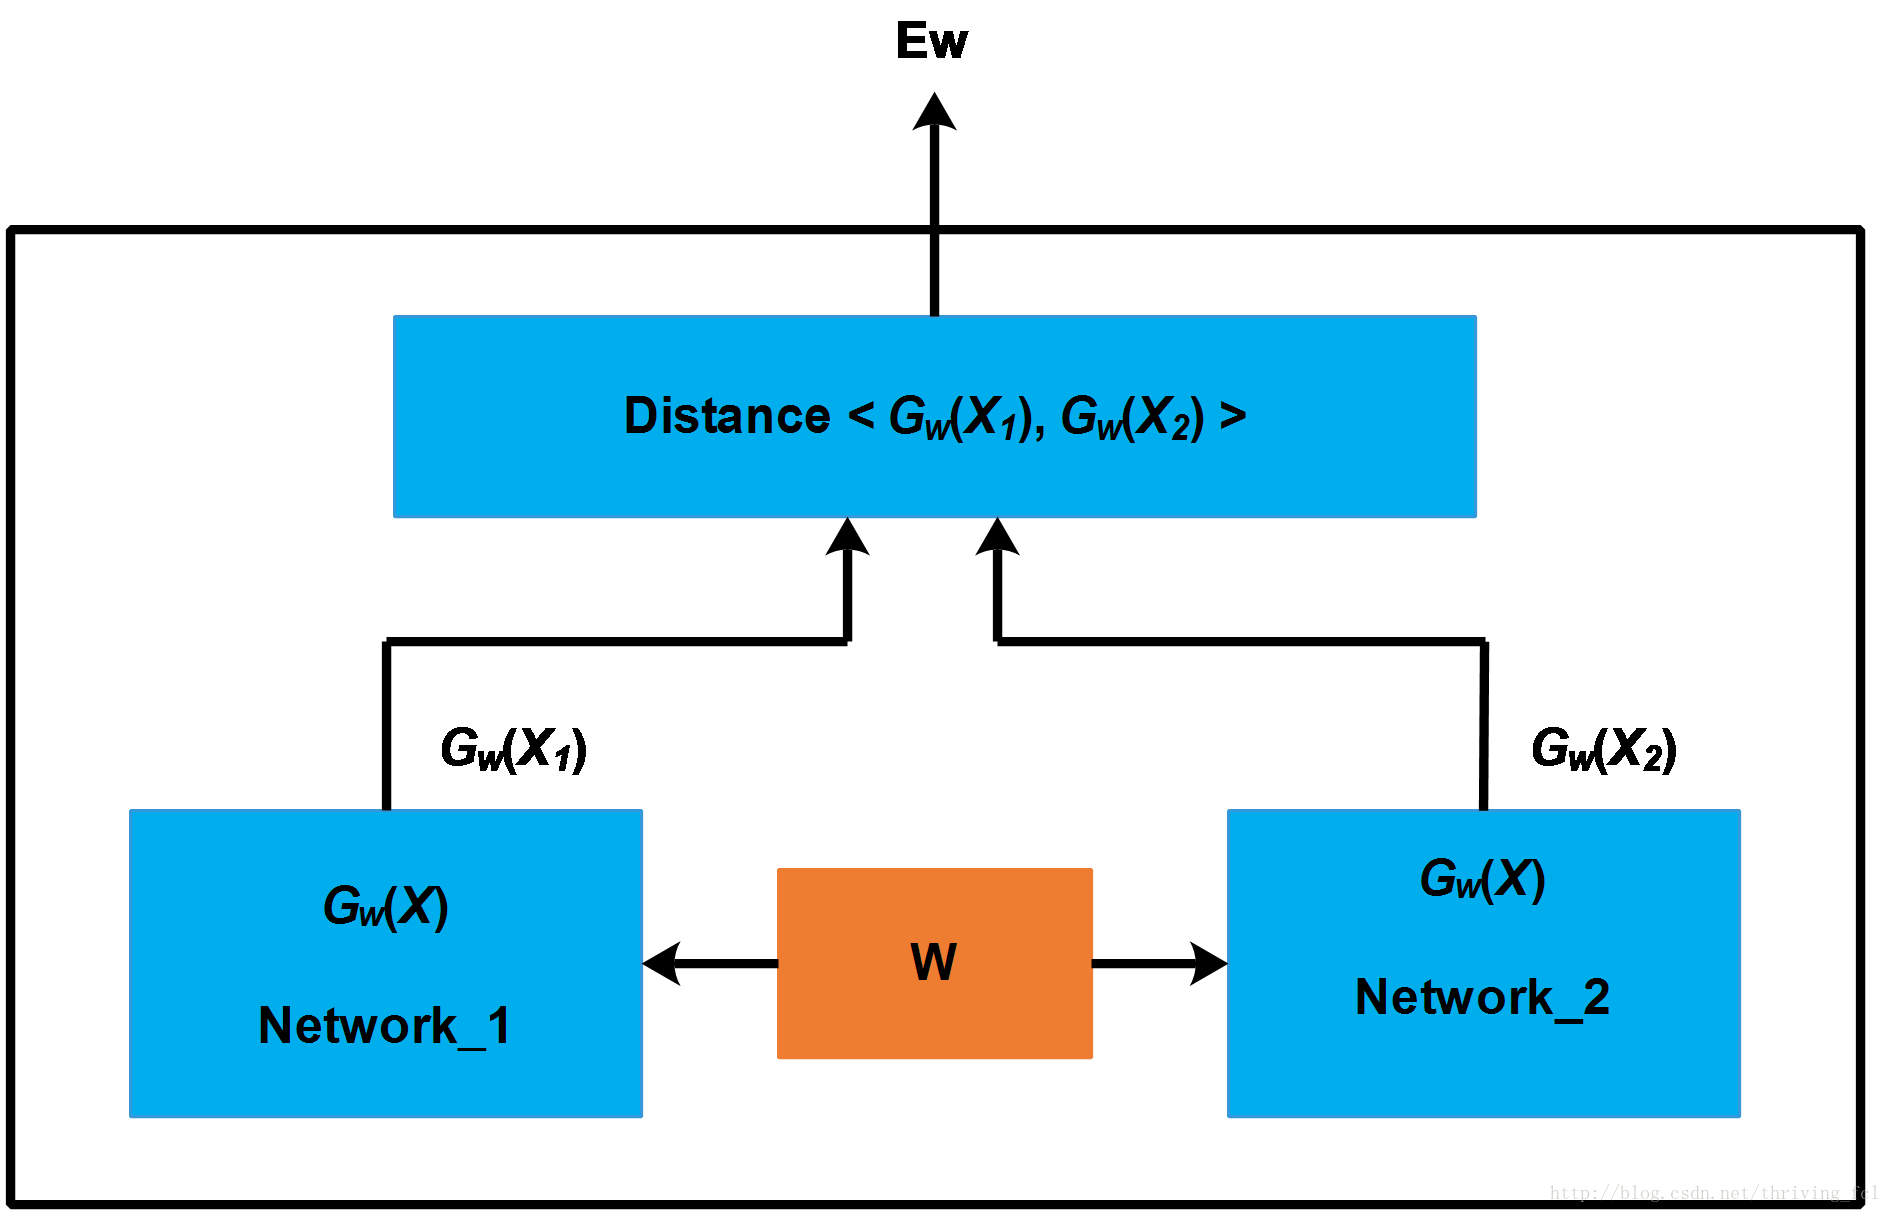
\includegraphics[width=0.6\textwidth]{Img/siamese-model.png}
    \bicaption{孪生网络模型架构}{Model architecture of Siamese Network}
    \label{fig:siamese-model}
\end{figure}
其中,Network\_1和Network\_2分别接收两个输入$X_1$与$X_2$,将其转换为向量$G_w(X_1)$与$G_w(X_2)$,再通过某种距离度量的方式计算两个输出向量的距离$E_w$。

本文由于以下原因采用孪生网络来解决样本数量的局限性。从直觉上讲,对于本任务而言,确定两个对话是否相似,要比为每个对话指定确切的类别更容易。另外,由于孪生网络将一对对话作为输入,因此数据集从元素级别转换为成对级别,可以通过对话之间的排列组合进行数据增强。

\section{本章小结}

本章主要针对在构建本文提出的基于孪生网络从大规模聊天记录中进行隐藏需求对话识别的方法时涉及到的相关概念和关键技术进行详细调研和总结。其中基于文本数据的需求发现主要包括基于手工设计规则和基于统计机器学习的方法,它们在不同的数据来源包括issue tracker、邮件列表等取得了较好的效果;聊天对话文本目前被广泛运用在软件工程中,并被当作丰富的信息来源;对于对话文本分类,本章介绍了常见的、效果稳定的文本分类模型;针对对话数据标注困难、样本少的情况,介绍了当前常见的包括孪生网络等的少样本学习技术。

